\lyxframe{Experimental Setup }

\begin{block}{Machine Parameter}
\begin{center}
\begin{tabular}{l|l}
\toprule
Prop                 & SNB16c       \\
\midrule
Micro-architecture    & Sandy-Bridge  \\
Sockets$\times$Cores & 2$\times$8   \\
Clock Rate           & 2.4GHz       \\
DRAM capacity        & 128GB        \\
DRAM Bandwidth       & 72GB/s      \\
Compiler       		 & Intel ``C'' compiler 15.0.0     \\
\bottomrule
\end{tabular}
\end{center}
\end{block}

\begin{block}{Fault Injection}
\begin{itemize}
\item Fault injection in reading graph data structure and $CC$ array.
\item Each fault injection read is independent
\item Normalized by number of edges in the network
\end{itemize}
\end{block}

\begin{itemize}
\item Test Network: $14^{th}$ DIMACS graph challenge
\end{itemize}
\lyxframeend{}

%%%%%%%%%%%%%%%%%%%%%%%%%%%%%%%%%%%%%%%%%%%%%%%%%%%%%%%%%

\lyxframe{Fault Free Execution Overhead }
\centering
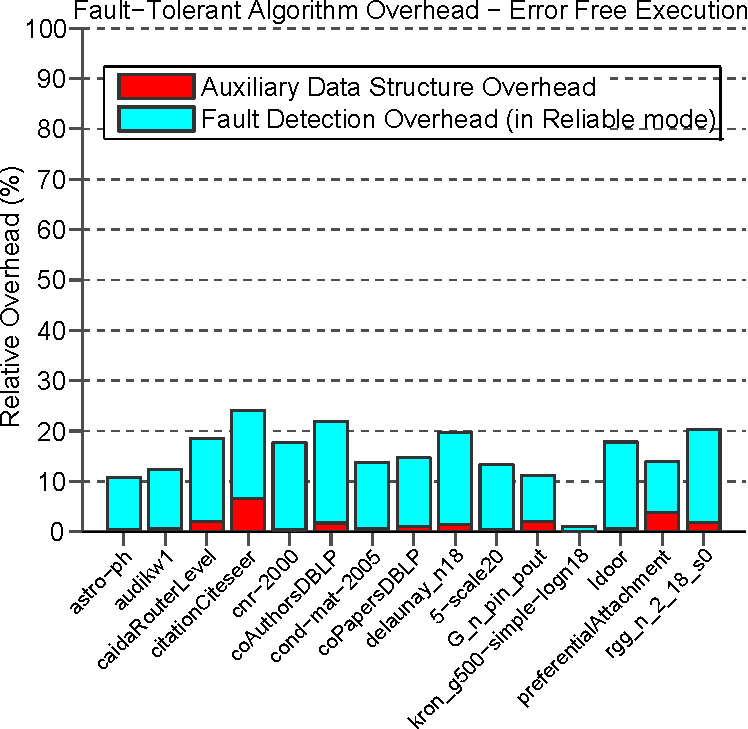
\includegraphics[height=.75\textheight]{plots/plot_zero_overhead-1}

\color{dpg} On an average 1.3\% overhead for maintaining additional data structure and 14\%
for fault detection.
\lyxframeend{}

%%%%%%%%%%%%%%%%%%%%%%%%%%%%%%%%%%%%%%%%%%%%%%%%%%%%%%%%%
\lyxframe{Overhead of Fault Tolerant Algorithm in the Presence of Faults }
\centering
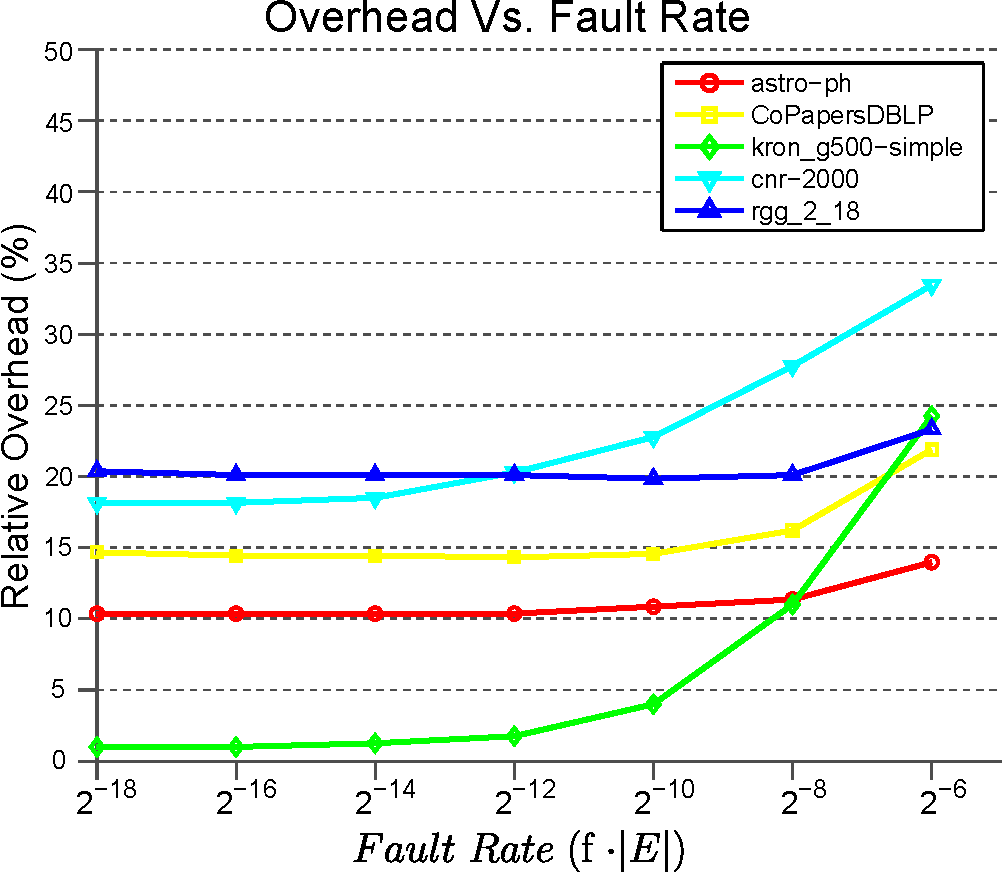
\includegraphics[height=.75\textheight]{plots/plot_overhead_fault-inked}



\lyxframeend{}

%%%%%%%%%%%%%%%%%%%%%%%%%%%%%%%%%%%%%%%%%%%%%%%%%%%%%%%%%
\lyxframe{Overhead of Fault Tolerant Algorithm in the Presence of Faults }
\centering
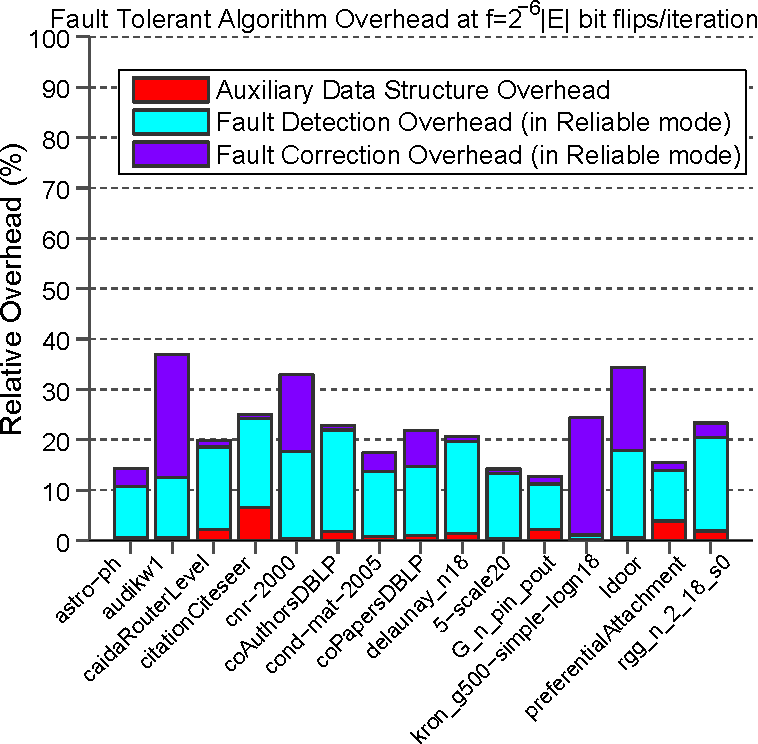
\includegraphics[height=.75\textheight]{plots/plot_overhead_2e6}

\color{dpg} Fault correction adds additional 9\% overhead at $2^{-6}$ bit flips per every memory access. 

\lyxframeend{}